% !TEX root = RRG_Technical_Appendix.tex
\documentclass[11pt,a4paper]{article}
\usepackage[margin=22mm,headheight=14pt]{geometry}
\usepackage{fontspec}
\setmainfont{Times New Roman}
\setsansfont{Arial}
\usepackage{amsmath,amssymb,float,graphicx,booktabs,longtable,array,caption,fancyhdr,xcolor,enumitem}
\usepackage[unicode,colorlinks=true,linkcolor=black,urlcolor=black,citecolor=black]{hyperref}
\definecolor{navy}{HTML}{171717}
\usepackage{titlesec}
\titleformat{\section}{\large\bfseries\color{navy}}{\thesection}{0.6em}{}
\titleformat{\subsection}{\normalsize\bfseries}{\thesubsection}{0.6em}{}
\titlespacing*{\section}{0pt}{10pt}{5pt}
\titlespacing*{\subsection}{0pt}{8pt}{4pt}
\setlength{\parindent}{0pt}
\setlength{\parskip}{5pt}
\linespread{1.04}
\setlength{\emergencystretch}{1.5em}
\captionsetup{font=small,labelfont=bf,skip=5pt}
\setlength{\tabcolsep}{5pt}
\renewcommand{\arraystretch}{1.13}
\pagestyle{fancy}\fancyhf{}
\fancyhead[L]{\small\sffamily RRG Sector Rotation | Empirical Analysis}
\fancyfoot[C]{\small\thepage}
\renewcommand{\headrulewidth}{0.3pt}
\setlist[itemize]{leftmargin=*,nosep,topsep=3pt}
\newcommand{\pp}{\,\text{pp}}

\hypersetup{pdftitle={RRG Sector Rotation: Technical Appendix},pdfauthor={}}
\renewcommand{\thesection}{\Alph{section}}
\renewcommand{\thetable}{\thesection\arabic{table}}
\renewcommand{\thefigure}{\thesection\arabic{figure}}
\begin{document}
\small
\setlength{\parskip}{4pt}
{\LARGE\bfseries RRG Sector Rotation}\par
{\large Technical Appendix: Data, Methods, and Supplementary Results}\par
{\small Companion to the five-page English report \hfill 7 November 2026}

This appendix uses the revised historical ETF pool throughout. Q denotes pure first-quadrant RRG; C denotes diffusion + RRG; M denotes sector momentum; E denotes equal-weight ETFs. Unless a table changes the setting, the sample is 28 December 2018--31 March 2026, with 220/60/20 trading-day signal windows, a maximum of six sectors, and 3 bp one-way fees. Percentages describe returns or risk; pp denotes percentage points. Tables and English vector figures are generated from the archived full-precision results. The conventions and comparison families match those of the main report.

\section{Data conventions and execution audit}
\subsection{Historical classification and product eligibility}
Historical membership is matched to its applicable interval. Missing classifications are excluded from the affected calculation. Free-float value is computed as reported free-float shares times the unadjusted stock close, with the source share-unit conversion. Its equivalence with Wind's free-float measure remains a data-definition issue. Stock-level diffusion uses unadjusted price changes. Sector signals use industry indices.

Stock-day coverage below is classified stock-days divided by observed stock-days; market-value coverage is their free-float value divided by the total available free-float value. The 2026 row ends on 31 March. Additional queries returned the existing 6,750 membership intervals and added zero intervals.

\begingroup\footnotesize\setlength{\tabcolsep}{4pt}\renewcommand{\arraystretch}{1.1}

\begin{longtable}{@{}lrrrr@{}}

\caption{Historical CITIC sector-membership coverage}\\\toprule

Year & Stock-days & Classified days & Day coverage & Value coverage\\\midrule\endfirsthead

\multicolumn{5}{l}{\textit{Table \thetable\ continued}}\\\toprule

Year & Stock-days & Classified days & Day coverage & Value coverage\\\midrule\endhead

\midrule\multicolumn{5}{r}{\textit{Continued on next page}}\\\endfoot\bottomrule\endlastfoot

2017 & 743,941 & 389,554 & 52.36\% & 37.64\%\\

2018 & 817,583 & 457,242 & 55.93\% & 35.55\%\\

2019 & 885,332 & 530,937 & 59.97\% & 41.89\%\\

2020 & 946,205 & 914,685 & 96.67\% & 98.66\%\\

2021 & 1,059,106 & 1,021,817 & 96.48\% & 99.13\%\\

2022 & 1,146,505 & 1,118,625 & 97.57\% & 99.42\%\\

2023 & 1,209,700 & 1,189,567 & 98.34\% & 99.59\%\\

2024 & 1,233,444 & 1,227,173 & 99.49\% & 99.86\%\\

2025 & 1,248,134 & 1,242,166 & 99.52\% & 99.88\%\\

2026 & 289,895 & 288,473 & 99.51\% & 99.85\%\\

\end{longtable}\endgroup

The product universe uses industry/theme labels in the current index directory. Matching exchange-traded codes to the corresponding off-exchange fund records repairs 248 metadata fields. Across the sample, 718 funds meet type/date eligibility; 54 are currently delisted and 35 previously enter an effective historical candidate pool. Current labels and incomplete historical tracking-index identities introduce classification uncertainty. At each formation, observed quotations, listing dates, holdings availability, overseas-holdings filtering, and same-index turnover selection determine eligibility. Twenty-day average turnover uses available history for more recent listings.

\clearpage\subsection{Holdings and delisted-fund treatment}
Fund exposures use holdings records announced by formation and historical sector membership. Partial disclosures retain original NAV weights. The fixed implementation deduplicates revised announcements using the latest announcement record, which can affect historical holdings availability. These conventions reduce certain information-timing risks while leaving incomplete disclosure and revision-history limitations.

Suspended or delisted holdings are valued at the last available adjusted price until modeled settlement. At the first monthly formation on or after delisting, the latest NAV already announced by formation, multiplied by the historical adjustment factor, determines estimated proceeds on the next trading day; fees apply. Plans cover 34 candidates. Main-setting E has 25 estimated settlements; Q, C and M each have zero. In the parameter grid, M at 260/6 and 260/8 has one each. Actual liquidation dates and cash receipts may differ.

\subsection{Research-report reconstruction and audit scope}
The source report uses Wind and Gildata. This study uses an authorized compatible interface and a reconstructed industry/theme ETF pool. The following difference describes the aggregate effect of data, universe and implementation conventions.

\begingroup\footnotesize\setlength{\tabcolsep}{4pt}\renewcommand{\arraystretch}{1.1}

\begin{longtable}{@{}lrr@{}}

\caption{Composite ETF strategy: published and reconstructed performance}\\\toprule

Metric & Published & Reconstructed\\\midrule\endfirsthead

\multicolumn{3}{l}{\textit{Table \thetable\ continued}}\\\toprule

Metric & Published & Reconstructed\\\midrule\endhead

\midrule\multicolumn{3}{r}{\textit{Continued on next page}}\\\endfoot\bottomrule\endlastfoot

Annualized return & 21.51\% & 18.95\%\\

Annualized volatility & 24.93\% & 27.02\%\\

Maximum drawdown & $-34.98\%$ & $-38.40\%$\\

Sharpe & 0.800 & 0.778\\

Calmar & 0.620 & 0.493\\

\end{longtable}\endgroup

Archived validation records report successful cash, fee, ending-value, next-open and post-settlement checks for all 43 cost/grid runs. Four main daily NAV paths reconcile with the prior revised-pool run; the three 220/6 grid paths reconcile with their corresponding main paths. These are accounting and implementation checks conditional on the inputs. Continuous units, proportional fees and adjusted opening prices are used. Lot sizes, minimum commissions and capital-specific market impact require further implementation work.

\clearpage\section{Signal definitions, optimizer, and performance measures}\setcounter{table}{0}\setcounter{figure}{0}

Let $P_{i,t}$ denote the sector price index, $B_t$ the daily-rebalanced equal-weight 28-sector benchmark NAV, and $\operatorname{MA}_{20}$ a trailing 20-trading-day simple average. The adopted fixed code calculates
\begin{align*}
B_t&=B_{t-1}\left(1+\frac{1}{n_t}\sum_{i\in I_t}\left(\frac{P_{i,t}}{P_{i,t-1}}-1\right)\right),\\
RS_{i,t}&=100P_{i,t}/B_t,\\
R_{i,t}&=\operatorname{MA}_{20}\left(100RS_{i,t}/RS_{i,t-L}\right),\\
M_{i,t}&=\operatorname{MA}_{20}\left(100R_{i,t}/R_{i,t-60}\right).
\end{align*}
Here $I_t$ is the set with available returns and $n_t=|I_t|$. Main $L=220$. Q selects up to $N=6$ sectors with $R>100$ and $M>100$, ranked by $\sqrt{(R-100)^2+(M-100)^2}$. Coordinate values exactly equal to 100 are left outside the strict quadrant inequalities. M ranks sectors by $P_{i,t}/P_{i,t-L}-1$.

For sector $i$, diffusion is the 20-day smoothed fraction of available free-float value in constituent stocks with positive $L$-day price changes:
\[
D_{i,t}=\operatorname{MA}_{20}\left[\frac{\sum_{j\in i}v_{j,t}\,\mathbf{1}(p_{j,t}/p_{j,t-L}-1>0)}{\sum_{j\in i}v_{j,t}}\right].
\]
C ranks diffusion, takes the top $N$ sectors, and retains those in the first or second quadrant. Its selection stops at that filter, so actual counts vary. Valid denominators with zero rising constituents give zero diffusion. The repair resides in the data adapter.

Let $E_{f,i}$ be visible industry exposure per ETF NAV, $s_i$ the binary selected-sector indicator, and $k=\sum_i s_i$. The three active schemes share:
\begin{align*}
\max_{w}\quad &\sum_f w_f\sum_i E_{f,i}s_i\\
\text{subject to}\quad &\sum_f w_f=1,\quad 0\leq w_f\leq1,\\
&\sum_f w_fE_{f,i}\leq1/k\quad\text{for each selected sector }i.
\end{align*}
This caps selected-sector exposure while allowing unequal ETF weights, exposure to other sectors and concentrated ETF holdings. The main Q portfolio's time-average largest actual ETF weight is 42.72\%; for C it is 50.50\%. E rebalances the available exposure-matrix fund pool to equal ETF weights.

With $T=1756$, annualized return is $(V_T/V_0)^{252/T}-1$. Volatility is the daily-return standard deviation times $\sqrt{252}$. Sharpe is daily mean return divided by its standard deviation times $\sqrt{252}$, with zero risk-free rate. Maximum drawdown is the minimum of $V_t/\max_{u\leq t}V_u-1$. Calmar divides annualized return by absolute maximum drawdown. Two-way turnover adds purchases and sales divided by prior NAV and annualizes by $252/T$.

\begingroup\footnotesize\setlength{\tabcolsep}{4pt}\renewcommand{\arraystretch}{1.1}

\begin{longtable}{@{}lrrrr@{}}

\caption{Supplementary main-setting implementation statistics}\\\toprule

Strategy & Calmar & Two-way turnover & Mean largest ETF & Ending CNY m\\\midrule\endfirsthead

\multicolumn{5}{l}{\textit{Table \thetable\ continued}}\\\toprule

Strategy & Calmar & Two-way turnover & Mean largest ETF & Ending CNY m\\\midrule\endhead

\midrule\multicolumn{5}{r}{\textit{Continued on next page}}\\\endfoot\bottomrule\endlastfoot

Q & 0.550 & 14.97 & 42.72\% & 46.36\\

C & 0.493 & 15.21 & 50.50\% & 33.51\\

M & 0.473 & 12.56 & 41.95\% & 39.58\\

E & 0.261 & 1.77 & 0.97\% & 19.57\\

\end{longtable}\endgroup

\clearpage\section{Time variation and return concentration}\setcounter{table}{0}\setcounter{figure}{0}

\begingroup\footnotesize\setlength{\tabcolsep}{4pt}\renewcommand{\arraystretch}{1.1}

\begin{longtable}{@{}lrrrr@{}}

\caption{Calendar-period net returns}\\\toprule

Period & Q & C & M & E\\\midrule\endfirsthead

\multicolumn{5}{l}{\textit{Table \thetable\ continued}}\\\toprule

Period & Q & C & M & E\\\midrule\endhead

\midrule\multicolumn{5}{r}{\textit{Continued on next page}}\\\endfoot\bottomrule\endlastfoot

2019 & 57.45\% & 27.27\% & 55.82\% & 31.10\%\\

2020 & 93.54\% & 69.09\% & 67.06\% & 34.30\%\\

2021 & 26.52\% & 27.60\% & 20.66\% & 7.60\%\\

2022 & -16.47\% & -1.67\% & -9.90\% & -20.58\%\\

2023 & -16.55\% & -21.07\% & -21.34\% & -7.31\%\\

2024 & 19.22\% & 10.93\% & 16.88\% & 10.61\%\\

2025 & 37.59\% & 30.33\% & 41.80\% & 29.02\%\\

2026 Q1 & 5.15\% & 8.77\% & 7.30\% & -1.66\%\\

\end{longtable}\endgroup

The 2018 observation is 28 December only, before first execution; all four returns are zero. The 2026 Q1 observation is an unannualized three-month return.

\begin{figure}[H]\centering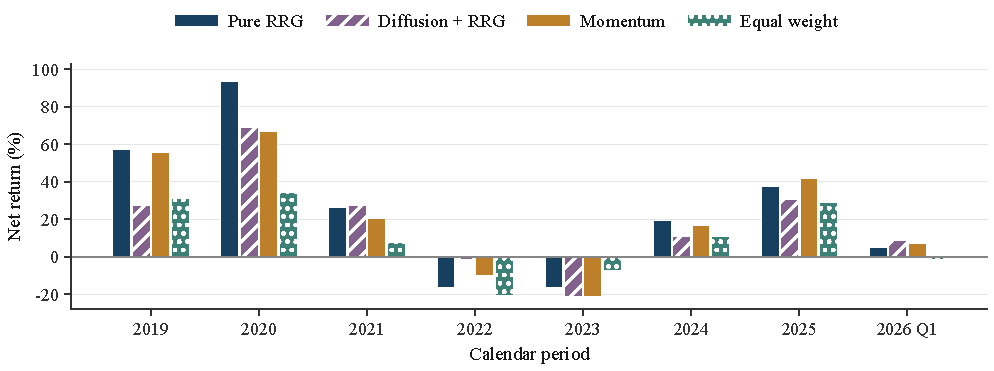
\includegraphics[width=\linewidth,height=.37\textheight,keepaspectratio]{figures/05_annual_returns.pdf}\caption{Calendar-period net returns after 3 bp one-way costs. The final observation covers January--March 2026 and is presented as an unannualized quarterly return.}\end{figure}

\begingroup\footnotesize\setlength{\tabcolsep}{4pt}\renewcommand{\arraystretch}{1.1}

\begin{longtable}{@{}lrrrrrr@{}}

\caption{Rolling 12-month descriptive statistics}\\\toprule

Strategy & Windows & Ranked first & Positive & Median & Worst & Best\\\midrule\endfirsthead

\multicolumn{7}{l}{\textit{Table \thetable\ continued}}\\\toprule

Strategy & Windows & Ranked first & Positive & Median & Worst & Best\\\midrule\endhead

\midrule\multicolumn{7}{r}{\textit{Continued on next page}}\\\endfoot\bottomrule\endlastfoot

Q & 76 & 29 & 50 & 20.22\% & -23.81\% & 93.54\%\\

C & 76 & 18 & 51 & 21.56\% & -22.77\% & 72.01\%\\

M & 76 & 13 & 52 & 14.30\% & -25.07\% & 71.10\%\\

E & 76 & 16 & 48 & 9.41\% & -24.52\% & 53.33\%\\

\end{longtable}\endgroup

Adjacent rolling windows overlap. Q exceeds M, C and E in 47, 53 and 55 windows, respectively, based on the archived rolling monthly series.

\begin{figure}[H]\centering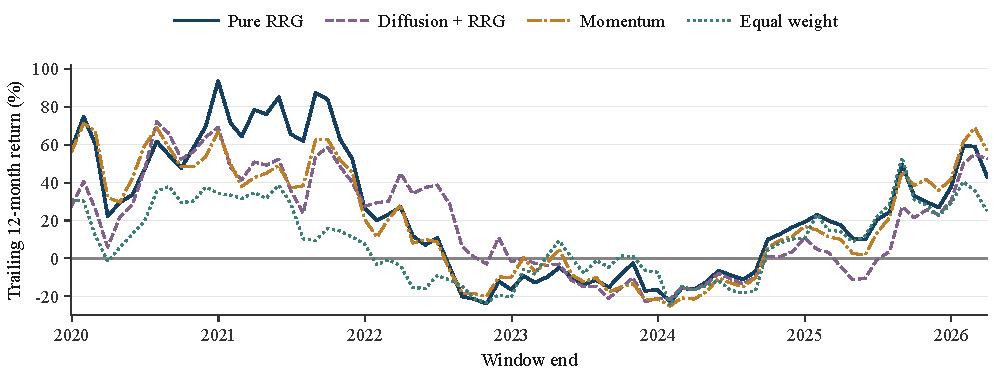
\includegraphics[width=\linewidth,height=.37\textheight,keepaspectratio]{figures/06_rolling_returns.pdf}\caption{Trailing 12-month net returns. Each series comprises 76 monthly observations; adjacent windows share eleven months. The horizontal reference line denotes zero return.}\end{figure}

\begingroup\footnotesize\setlength{\tabcolsep}{4pt}\renewcommand{\arraystretch}{1.1}

\begin{longtable}{@{}lrrrr@{}}

\caption{Month-concentration diagnostic}\\\toprule

Strategy & Positive/negative & Top-3 log growth & Best-1 flat CAGR & Best-3 flat CAGR\\\midrule\endfirsthead

\multicolumn{5}{l}{\textit{Table \thetable\ continued}}\\\toprule

Strategy & Positive/negative & Top-3 log growth & Best-1 flat CAGR & Best-3 flat CAGR\\\midrule\endhead

\midrule\multicolumn{5}{r}{\textit{Continued on next page}}\\\endfoot\bottomrule\endlastfoot

Q & 46/41 & 34.92\% & 20.97\% & 15.40\%\\

C & 48/39 & 46.37\% & 15.51\% & 9.75\%\\

M & 47/40 & 35.11\% & 18.92\% & 13.67\%\\

E & 49/38 & 73.31\% & 6.90\% & 2.61\%\\

\end{longtable}\endgroup

Top-three growth share divides the sum of the best three monthly log returns by full-period log growth. Flat-month scenarios set each strategy's own best one or three monthly returns to zero while retaining sample length. They diagnose retrospective concentration.

\begingroup\footnotesize\setlength{\tabcolsep}{4pt}\renewcommand{\arraystretch}{1.1}

\begin{longtable}{@{}lrrrr@{}}

\caption{Best and worst return months}\\\toprule

Strategy & Best month & Return & Worst month & Return\\\midrule\endfirsthead

\multicolumn{5}{l}{\textit{Table \thetable\ continued}}\\\toprule

Strategy & Best month & Return & Worst month & Return\\\midrule\endhead

\midrule\multicolumn{5}{r}{\textit{Continued on next page}}\\\endfoot\bottomrule\endlastfoot

Q & 2020-12 & 23.01\% & 2020-03 & -12.65\%\\

C & 2021-08 & 22.73\% & 2020-03 & -12.97\%\\

M & 2025-08 & 18.33\% & 2020-03 & -13.37\%\\

E & 2024-09 & 22.95\% & 2024-01 & -12.31\%\\

\end{longtable}\endgroup

\clearpage\section{Cost, parameter, and statistical robustness}\setcounter{table}{0}\setcounter{figure}{0}

\subsection{Cost and parameter sensitivity}
Each cost case replays the same target rules with uniform one-way fees of 3, 5, 10 or 20 bp and zero additional slippage. The parameter grid changes $L\in\{180,220,260\}$ and $N\in\{4,6,8\}$. The 60-day momentum and 20-day smoothing windows remain fixed. C changes both diffusion and relative-strength lookback with $L$. E retains its fixed main return. All results use the same observed historical sample.

\begingroup\footnotesize\setlength{\tabcolsep}{4pt}\renewcommand{\arraystretch}{1.1}

\begin{longtable}{@{}lrrrrrr@{}}

\caption{All 16 transaction-cost cases}\\\toprule

Strategy & bp & Ann. return & Max. DD & Volatility & Sharpe & Calmar\\\midrule\endfirsthead

\multicolumn{7}{l}{\textit{Table \thetable\ continued}}\\\toprule

Strategy & bp & Ann. return & Max. DD & Volatility & Sharpe & Calmar\\\midrule\endhead

\midrule\multicolumn{7}{r}{\textit{Continued on next page}}\\\endfoot\bottomrule\endlastfoot

Q & 3 & 24.62\% & -44.76\% & 26.36\% & 0.967 & 0.550\\

C & 3 & 18.95\% & -38.40\% & 27.02\% & 0.778 & 0.493\\

M & 3 & 21.83\% & -46.19\% & 25.92\% & 0.892 & 0.473\\

E & 3 & 10.12\% & -38.78\% & 19.68\% & 0.588 & 0.261\\

Q & 5 & 24.25\% & -45.11\% & 26.35\% & 0.956 & 0.538\\

C & 5 & 18.59\% & -38.90\% & 27.01\% & 0.767 & 0.478\\

M & 5 & 21.52\% & -46.57\% & 25.91\% & 0.883 & 0.462\\

E & 5 & 10.08\% & -38.81\% & 19.68\% & 0.587 & 0.260\\

Q & 10 & 23.32\% & -45.98\% & 26.34\% & 0.928 & 0.507\\

C & 10 & 17.69\% & -40.11\% & 26.99\% & 0.739 & 0.441\\

M & 10 & 20.77\% & -47.49\% & 25.90\% & 0.859 & 0.437\\

E & 10 & 9.99\% & -38.89\% & 19.68\% & 0.582 & 0.257\\

Q & 20 & 21.49\% & -47.69\% & 26.33\% & 0.871 & 0.451\\

C & 20 & 15.91\% & -42.78\% & 26.96\% & 0.683 & 0.372\\

M & 20 & 19.27\% & -49.28\% & 25.87\% & 0.811 & 0.391\\

E & 20 & 9.80\% & -39.10\% & 19.67\% & 0.574 & 0.251\\

\end{longtable}\endgroup

\begin{figure}[H]\centering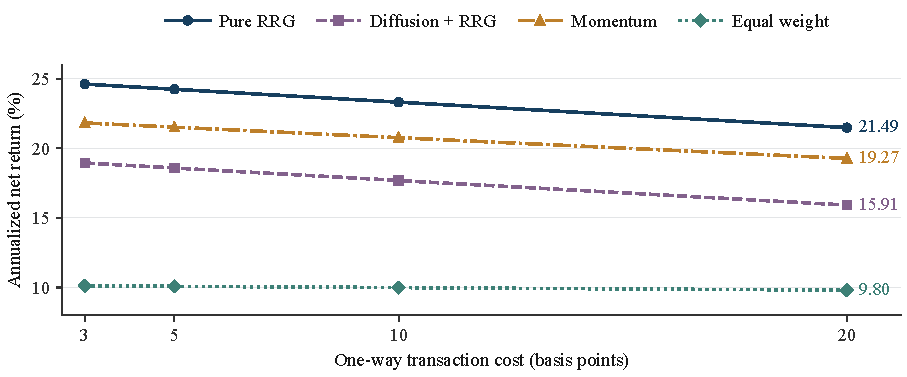
\includegraphics[width=\linewidth,height=.37\textheight,keepaspectratio]{figures/02_cost.pdf}\caption{Transaction-cost sensitivity. Target portfolios are replayed at each uniform one-way cost. Labels at 20 bp report the resulting annualized net returns (\%).}\end{figure}

\begingroup\footnotesize\setlength{\tabcolsep}{4pt}\renewcommand{\arraystretch}{1.1}

\clearpage
\begin{longtable}{@{}lrrrrrrr@{}}

\caption{All 27 active-strategy parameter cases}\\\toprule

Strategy & $L$ & $N$ & Ann. return & Max. DD & Volatility & Sharpe & Calmar\\\midrule\endfirsthead

\multicolumn{8}{l}{\textit{Table \thetable\ continued}}\\\toprule

Strategy & $L$ & $N$ & Ann. return & Max. DD & Volatility & Sharpe & Calmar\\\midrule\endhead

\midrule\multicolumn{8}{r}{\textit{Continued on next page}}\\\endfoot\bottomrule\endlastfoot

Q & 180 & 4 & 20.14\% & -47.18\% & 27.23\% & 0.811 & 0.427\\

C & 180 & 4 & 16.91\% & -43.05\% & 27.59\% & 0.705 & 0.393\\

M & 180 & 4 & 19.59\% & -55.43\% & 28.29\% & 0.774 & 0.353\\

Q & 180 & 6 & 19.40\% & -44.01\% & 25.54\% & 0.822 & 0.441\\

C & 180 & 6 & 12.07\% & -35.27\% & 26.25\% & 0.566 & 0.342\\

M & 180 & 6 & 16.76\% & -46.96\% & 25.30\% & 0.739 & 0.357\\

Q & 180 & 8 & 16.27\% & -39.06\% & 25.01\% & 0.728 & 0.417\\

C & 180 & 8 & 14.04\% & -41.86\% & 25.56\% & 0.642 & 0.335\\

M & 180 & 8 & 13.58\% & -48.57\% & 24.23\% & 0.647 & 0.280\\

Q & 220 & 4 & 17.42\% & -48.83\% & 27.76\% & 0.718 & 0.357\\

C & 220 & 4 & 23.98\% & -44.83\% & 29.91\% & 0.869 & 0.535\\

M & 220 & 4 & 18.81\% & -48.94\% & 26.86\% & 0.776 & 0.384\\

Q & 220 & 6 & 24.62\% & -44.76\% & 26.36\% & 0.967 & 0.550\\

C & 220 & 6 & 18.95\% & -38.40\% & 27.02\% & 0.778 & 0.493\\

M & 220 & 6 & 21.83\% & -46.19\% & 25.92\% & 0.892 & 0.473\\

Q & 220 & 8 & 23.95\% & -37.57\% & 25.65\% & 0.966 & 0.637\\

C & 220 & 8 & 20.16\% & -42.93\% & 26.27\% & 0.831 & 0.470\\

M & 220 & 8 & 19.94\% & -44.49\% & 25.11\% & 0.850 & 0.448\\

Q & 260 & 4 & 12.73\% & -57.89\% & 28.25\% & 0.566 & 0.220\\

C & 260 & 4 & 15.08\% & -58.74\% & 28.93\% & 0.631 & 0.257\\

M & 260 & 4 & 15.50\% & -54.11\% & 27.67\% & 0.660 & 0.287\\

Q & 260 & 6 & 21.14\% & -54.01\% & 27.19\% & 0.842 & 0.391\\

C & 260 & 6 & 16.62\% & -48.01\% & 27.37\% & 0.699 & 0.346\\

M & 260 & 6 & 19.38\% & -48.48\% & 26.54\% & 0.801 & 0.400\\

Q & 260 & 8 & 19.16\% & -55.91\% & 26.86\% & 0.787 & 0.343\\

C & 260 & 8 & 13.71\% & -56.65\% & 27.54\% & 0.605 & 0.242\\

M & 260 & 8 & 19.80\% & -46.51\% & 25.79\% & 0.830 & 0.426\\

\end{longtable}\endgroup

Matched parameters mean the same lookback and nominal sector cap; realized counts may differ. Q exceeds matched M in six cases and matched C in seven. It exceeds fixed 220/6 M in two cases. Q is above E in all nine cases. These comparisons answer different allocation questions.

\subsection{Paired mean-return inference}
Tests use the 87 non-overlapping complete months from January 2019 through March 2026. For paired return differences, HAC inference uses lag three as the main choice, small-sample correction and a two-sided t approximation; lags one and six are sensitivity checks. Confidence intervals are individual 95\% intervals. Holm adjustment is applied separately to six primary, 24 cost and 54 grid comparisons. Every adjusted p-value in those three families exceeds 0.05. These families cover the specified current tests; historical research choices add further selection uncertainty.

\begingroup\footnotesize\setlength{\tabcolsep}{4pt}\renewcommand{\arraystretch}{1.1}

\begin{longtable}{@{}lrrrr@{}}

\caption{Six primary HAC(3) paired comparisons}\\\toprule

Pair & Mean gap pp & 95\% CI pp & Raw $p$ & Holm $p$\\\midrule\endfirsthead

\multicolumn{5}{l}{\textit{Table \thetable\ continued}}\\\toprule

Pair & Mean gap pp & 95\% CI pp & Raw $p$ & Holm $p$\\\midrule\endhead

\midrule\multicolumn{5}{r}{\textit{Continued on next page}}\\\endfoot\bottomrule\endlastfoot

Q--C & 0.395 & [-0.404, 1.194] & 0.3284 & 0.9852\\

Q--M & 0.198 & [-0.342, 0.739] & 0.4681 & 0.9852\\

Q--E & 1.076 & [0.199, 1.953] & 0.0168 & 0.1010\\

C--M & -0.197 & [-0.896, 0.503] & 0.5773 & 0.9852\\

C--E & 0.681 & [-0.345, 1.706] & 0.1904 & 0.7615\\

M--E & 0.878 & [-0.062, 1.817] & 0.0667 & 0.3335\\

\end{longtable}\endgroup

\begin{figure}[H]\centering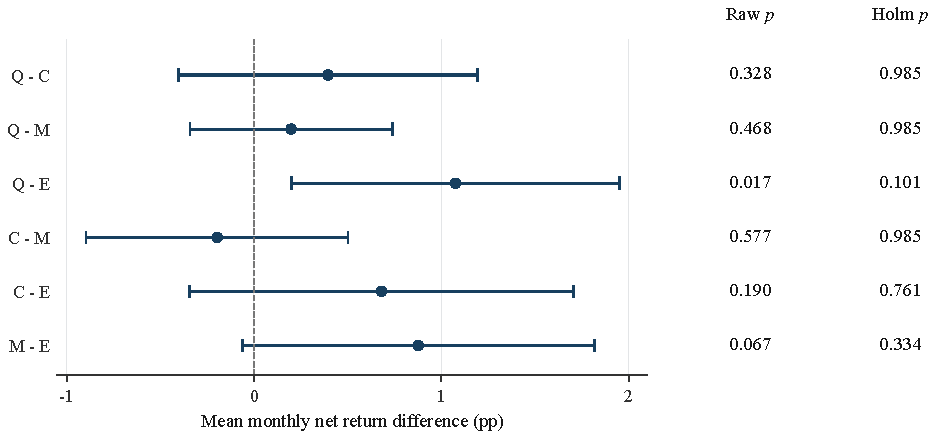
\includegraphics[width=\linewidth,height=.37\textheight,keepaspectratio]{figures/04_significance.pdf}\caption{Paired mean monthly net-return differences. Points denote estimates and bars individual 95\% HAC(3) confidence intervals. Raw p-values and Holm-adjusted p-values refer to the six primary comparisons. Units are percentage points.}\end{figure}

\begingroup\footnotesize\setlength{\tabcolsep}{4pt}\renewcommand{\arraystretch}{1.1}

\begin{longtable}{@{}lrrrr@{}}

\caption{HAC lag sensitivity: all 18 cases}\\\toprule

Lag & Pair & Mean gap pp & 95\% CI pp & Raw $p$\\\midrule\endfirsthead

\multicolumn{5}{l}{\textit{Table \thetable\ continued}}\\\toprule

Lag & Pair & Mean gap pp & 95\% CI pp & Raw $p$\\\midrule\endhead

\midrule\multicolumn{5}{r}{\textit{Continued on next page}}\\\endfoot\bottomrule\endlastfoot

1 & Q--C & 0.395 & [-0.322, 1.113] & 0.2768\\

3 & Q--C & 0.395 & [-0.404, 1.194] & 0.3284\\

6 & Q--C & 0.395 & [-0.482, 1.272] & 0.3729\\

1 & Q--M & 0.198 & [-0.353, 0.749] & 0.4763\\

3 & Q--M & 0.198 & [-0.342, 0.739] & 0.4681\\

6 & Q--M & 0.198 & [-0.354, 0.750] & 0.4772\\

1 & Q--E & 1.076 & [0.106, 2.045] & 0.0301\\

3 & Q--E & 1.076 & [0.199, 1.953] & 0.0168\\

6 & Q--E & 1.076 & [0.234, 1.917] & 0.0128\\

1 & C--M & -0.197 & [-0.932, 0.539] & 0.5960\\

3 & C--M & -0.197 & [-0.896, 0.503] & 0.5773\\

6 & C--M & -0.197 & [-0.945, 0.551] & 0.6021\\

1 & C--E & 0.681 & [-0.388, 1.750] & 0.2090\\

3 & C--E & 0.681 & [-0.345, 1.706] & 0.1904\\

6 & C--E & 0.681 & [-0.371, 1.732] & 0.2016\\

1 & M--E & 0.878 & [-0.138, 1.893] & 0.0895\\

3 & M--E & 0.878 & [-0.062, 1.817] & 0.0667\\

6 & M--E & 0.878 & [0.012, 1.743] & 0.0471\\

\end{longtable}\endgroup

\begingroup\footnotesize\setlength{\tabcolsep}{4pt}\renewcommand{\arraystretch}{1.1}

\begin{longtable}{@{}lrrrrr@{}}

\caption{Cost-family paired comparisons: all 24 cases}\\\toprule

bp & Pair & Mean gap pp & 95\% CI pp & Raw $p$ & Holm $p$\\\midrule\endfirsthead

\multicolumn{6}{l}{\textit{Table \thetable\ continued}}\\\toprule

bp & Pair & Mean gap pp & 95\% CI pp & Raw $p$ & Holm $p$\\\midrule\endhead

\midrule\multicolumn{6}{r}{\textit{Continued on next page}}\\\endfoot\bottomrule\endlastfoot

3 & Q--C & 0.395 & [-0.404, 1.194] & 0.3284 & 1.0000\\

3 & Q--M & 0.198 & [-0.342, 0.739] & 0.4681 & 1.0000\\

3 & Q--E & 1.076 & [0.199, 1.953] & 0.0168 & 0.4038\\

3 & C--M & -0.197 & [-0.896, 0.503] & 0.5773 & 1.0000\\

3 & C--E & 0.681 & [-0.345, 1.706] & 0.1904 & 1.0000\\

3 & M--E & 0.878 & [-0.062, 1.817] & 0.0667 & 1.0000\\

5 & Q--C & 0.395 & [-0.404, 1.195] & 0.3282 & 1.0000\\

5 & Q--M & 0.194 & [-0.346, 0.734] & 0.4768 & 1.0000\\

5 & Q--E & 1.054 & [0.177, 1.931] & 0.0191 & 0.4396\\

5 & C--M & -0.201 & [-0.901, 0.498] & 0.5686 & 1.0000\\

5 & C--E & 0.658 & [-0.367, 1.684] & 0.2054 & 1.0000\\

5 & M--E & 0.860 & [-0.080, 1.800] & 0.0724 & 1.0000\\

10 & Q--C & 0.396 & [-0.404, 1.197] & 0.3278 & 1.0000\\

10 & Q--M & 0.183 & [-0.354, 0.721] & 0.4992 & 1.0000\\

10 & Q--E & 0.999 & [0.122, 1.876] & 0.0260 & 0.5726\\

10 & C--M & -0.213 & [-0.914, 0.488] & 0.5473 & 1.0000\\

10 & C--E & 0.603 & [-0.424, 1.629] & 0.2463 & 1.0000\\

10 & M--E & 0.816 & [-0.125, 1.756] & 0.0883 & 1.0000\\

20 & Q--C & 0.398 & [-0.405, 1.202] & 0.3272 & 1.0000\\

20 & Q--M & 0.162 & [-0.371, 0.695] & 0.5464 & 1.0000\\

20 & Q--E & 0.891 & [0.015, 1.768] & 0.0464 & 0.9738\\

20 & C--M & -0.236 & [-0.938, 0.467] & 0.5061 & 1.0000\\

20 & C--E & 0.493 & [-0.535, 1.521] & 0.3433 & 1.0000\\

20 & M--E & 0.729 & [-0.213, 1.671] & 0.1278 & 1.0000\\

\end{longtable}\endgroup

\begingroup\footnotesize\setlength{\tabcolsep}{4pt}\renewcommand{\arraystretch}{1.1}

\begin{longtable}{@{}lrrrrrr@{}}

\caption{Parameter-family paired comparisons: all 54 cases}\\\toprule

$L$ & $N$ & Pair & Mean gap pp & 95\% CI pp & Raw $p$ & Holm $p$\\\midrule\endfirsthead

\multicolumn{7}{l}{\textit{Table \thetable\ continued}}\\\toprule

$L$ & $N$ & Pair & Mean gap pp & 95\% CI pp & Raw $p$ & Holm $p$\\\midrule\endhead

\midrule\multicolumn{7}{r}{\textit{Continued on next page}}\\\endfoot\bottomrule\endlastfoot

180 & 4 & Q--C & 0.179 & [-0.683, 1.041] & 0.6812 & 1.0000\\

180 & 4 & Q--M & 0.044 & [-0.741, 0.828] & 0.9122 & 1.0000\\

180 & 4 & C--M & -0.135 & [-1.197, 0.927] & 0.8010 & 1.0000\\

180 & 4 & Q--E & 0.804 & [-0.171, 1.780] & 0.1050 & 1.0000\\

180 & 4 & C--E & 0.625 & [-0.386, 1.637] & 0.2225 & 1.0000\\

180 & 4 & M--E & 0.760 & [-0.473, 1.994] & 0.2238 & 1.0000\\

180 & 6 & Q--C & 0.512 & [-0.237, 1.261] & 0.1777 & 1.0000\\

180 & 6 & Q--M & 0.226 & [-0.605, 1.057] & 0.5901 & 1.0000\\

180 & 6 & C--M & -0.286 & [-0.968, 0.396] & 0.4066 & 1.0000\\

180 & 6 & Q--E & 0.725 & [-0.127, 1.577] & 0.0942 & 1.0000\\

180 & 6 & C--E & 0.213 & [-0.686, 1.112] & 0.6389 & 1.0000\\

180 & 6 & M--E & 0.499 & [-0.437, 1.435] & 0.2919 & 1.0000\\

180 & 8 & Q--C & 0.147 & [-0.383, 0.677] & 0.5820 & 1.0000\\

180 & 8 & Q--M & 0.238 & [-0.452, 0.929] & 0.4943 & 1.0000\\

180 & 8 & C--M & 0.091 & [-0.481, 0.663] & 0.7524 & 1.0000\\

180 & 8 & Q--E & 0.495 & [-0.269, 1.258] & 0.2016 & 1.0000\\

180 & 8 & C--E & 0.347 & [-0.478, 1.173] & 0.4055 & 1.0000\\

180 & 8 & M--E & 0.256 & [-0.524, 1.036] & 0.5156 & 1.0000\\

220 & 4 & Q--C & -0.479 & [-1.180, 0.221] & 0.1774 & 1.0000\\

220 & 4 & Q--M & -0.113 & [-0.762, 0.536] & 0.7300 & 1.0000\\

220 & 4 & C--M & 0.366 & [-0.472, 1.204] & 0.3873 & 1.0000\\

220 & 4 & Q--E & 0.611 & [-0.266, 1.489] & 0.1695 & 1.0000\\

220 & 4 & C--E & 1.091 & [-0.086, 2.267] & 0.0687 & 1.0000\\

220 & 4 & M--E & 0.724 & [-0.459, 1.908] & 0.2269 & 1.0000\\

220 & 6 & Q--C & 0.395 & [-0.404, 1.194] & 0.3284 & 1.0000\\

220 & 6 & Q--M & 0.198 & [-0.342, 0.739] & 0.4681 & 1.0000\\

220 & 6 & C--M & -0.197 & [-0.896, 0.503] & 0.5773 & 1.0000\\

220 & 6 & Q--E & 1.076 & [0.199, 1.953] & 0.0168 & 0.8918\\

220 & 6 & C--E & 0.681 & [-0.345, 1.706] & 0.1904 & 1.0000\\

220 & 6 & M--E & 0.878 & [-0.062, 1.817] & 0.0667 & 1.0000\\

220 & 8 & Q--C & 0.261 & [-0.214, 0.737] & 0.2774 & 1.0000\\

220 & 8 & Q--M & 0.276 & [-0.193, 0.744] & 0.2456 & 1.0000\\

220 & 8 & C--M & 0.014 & [-0.566, 0.595] & 0.9612 & 1.0000\\

220 & 8 & Q--E & 1.014 & [0.285, 1.743] & 0.0069 & 0.3741\\

220 & 8 & C--E & 0.753 & [-0.150, 1.655] & 0.1010 & 1.0000\\

220 & 8 & M--E & 0.738 & [-0.004, 1.480] & 0.0511 & 1.0000\\

260 & 4 & Q--C & -0.163 & [-0.919, 0.594] & 0.6706 & 1.0000\\

260 & 4 & Q--M & -0.178 & [-1.102, 0.746] & 0.7026 & 1.0000\\

260 & 4 & C--M & -0.016 & [-0.839, 0.808] & 0.9702 & 1.0000\\

260 & 4 & Q--E & 0.325 & [-0.551, 1.202] & 0.4628 & 1.0000\\

260 & 4 & C--E & 0.488 & [-0.729, 1.704] & 0.4276 & 1.0000\\

260 & 4 & M--E & 0.503 & [-0.761, 1.768] & 0.4311 & 1.0000\\

260 & 6 & Q--C & 0.336 & [-0.353, 1.024] & 0.3356 & 1.0000\\

260 & 6 & Q--M & 0.152 & [-0.613, 0.917] & 0.6937 & 1.0000\\

260 & 6 & C--M & -0.184 & [-0.817, 0.449] & 0.5657 & 1.0000\\

260 & 6 & Q--E & 0.895 & [-0.069, 1.859] & 0.0685 & 1.0000\\

260 & 6 & C--E & 0.559 & [-0.381, 1.500] & 0.2406 & 1.0000\\

260 & 6 & M--E & 0.743 & [-0.214, 1.700] & 0.1266 & 1.0000\\

260 & 8 & Q--C & 0.373 & [-0.155, 0.901] & 0.1636 & 1.0000\\

260 & 8 & Q--M & -0.001 & [-0.668, 0.667] & 0.9986 & 1.0000\\

260 & 8 & C--M & -0.374 & [-1.015, 0.267] & 0.2498 & 1.0000\\

260 & 8 & Q--E & 0.757 & [-0.212, 1.727] & 0.1241 & 1.0000\\

260 & 8 & C--E & 0.384 & [-0.507, 1.276] & 0.3935 & 1.0000\\

260 & 8 & M--E & 0.758 & [-0.142, 1.658] & 0.0978 & 1.0000\\

\end{longtable}\endgroup

\clearpage\subsection{Paired circular block bootstrap}
Monthly return pairs are resampled together in circular blocks of three or six months, with 10,000 repetitions and random seed 20261107. Centered two-sided bootstrap p-values refer to the mean monthly difference. The table separately reports the annualized compounded-return gap and its percentile interval, annualized with the original $252/1756$ exponent. This preserves the distinction between the two estimands.

\begingroup\footnotesize\setlength{\tabcolsep}{4pt}\renewcommand{\arraystretch}{1.1}

\begin{longtable}{@{}lrrrrr@{}}

\caption{All 12 bootstrap cases}\\\toprule

Pair & Block & Mean gap pp & Centered $p$ & CAGR gap pp & CAGR 95\% CI pp\\\midrule\endfirsthead

\multicolumn{6}{l}{\textit{Table \thetable\ continued}}\\\toprule

Pair & Block & Mean gap pp & Centered $p$ & CAGR gap pp & CAGR 95\% CI pp\\\midrule\endhead

\midrule\multicolumn{6}{r}{\textit{Continued on next page}}\\\endfoot\bottomrule\endlastfoot

Q--C & 3 & 0.395 & 0.3083 & 5.67 & [-5.331, 17.626]\\

Q--C & 6 & 0.395 & 0.3506 & 5.67 & [-6.350, 18.500]\\

Q--M & 3 & 0.198 & 0.4591 & 2.79 & [-4.846, 10.761]\\

Q--M & 6 & 0.198 & 0.4803 & 2.79 & [-4.850, 11.573]\\

Q--E & 3 & 1.076 & 0.0203 & 14.50 & [2.543, 29.729]\\

Q--E & 6 & 1.076 & 0.0099 & 14.50 & [3.139, 27.925]\\

C--M & 3 & -0.197 & 0.5620 & -2.88 & [-13.186, 6.771]\\

C--M & 6 & -0.197 & 0.5953 & -2.88 & [-14.022, 7.766]\\

C--E & 3 & 0.681 & 0.1964 & 8.83 & [-4.881, 24.950]\\

C--E & 6 & 0.681 & 0.1934 & 8.83 & [-4.863, 23.727]\\

M--E & 3 & 0.878 & 0.0733 & 11.71 & [-0.765, 27.464]\\

M--E & 6 & 0.878 & 0.0490 & 11.71 & [0.020, 25.390]\\

\end{longtable}\endgroup

\subsection{Investable-benchmark regressions}
For Q and C separately, monthly returns are regressed on a constant, M returns and E returns. Intercept inference uses HAC(3). This measures increment relative to two investable portfolio benchmarks; its interpretation remains conditional on their exposures.

\begingroup\footnotesize\setlength{\tabcolsep}{4pt}\renewcommand{\arraystretch}{1.1}

\begin{longtable}{@{}lrrrrr@{}}

\caption{Benchmark regressions}\\\toprule

Strategy & Intercept pp & 95\% CI pp & Raw $p$ & Holm $p$ & $R^2$\\\midrule\endfirsthead

\multicolumn{6}{l}{\textit{Table \thetable\ continued}}\\\toprule

Strategy & Intercept pp & 95\% CI pp & Raw $p$ & Holm $p$ & $R^2$\\\midrule\endhead

\midrule\multicolumn{6}{r}{\textit{Continued on next page}}\\\endfoot\bottomrule\endlastfoot

Q & 0.304 & [-0.160, 0.768] & 0.1956 & 0.3913 & 0.879\\

C & 0.066 & [-0.638, 0.770] & 0.8520 & 0.8520 & 0.759\\

\end{longtable}\endgroup

For Q, the M and E coefficients are 0.823 and 0.230; for C, they are 0.783 and 0.139. Sector, size and other factor risks remain part of the unexplained attribution question.

\clearpage\section{Fixed ten-month moving-average risk-control comparison}\setcounter{table}{0}\setcounter{figure}{0}

The common market gate compares the 28-sector benchmark at month-end with its trailing ten month-end average, including the current month. A value above the average retains the original ETF targets; other observations allocate to cash at the next trading-day open. Both variants share the gate, 3 bp fees, zero cash yield, and the same delisting conventions. The fixed ten-month rule adapts Faber's tactical-allocation approach.

For Q, the filter reduces annualized return by 8.28 pp and deepens maximum drawdown by 2.28 pp. For M, the corresponding changes are 8.67 pp and 7.77 pp. Average cash holdings are approximately 30.47\% for the filtered portfolios. Volatility and fees decline while their realized drawdown paths worsen.

\begingroup\footnotesize\setlength{\tabcolsep}{4pt}\renewcommand{\arraystretch}{1.1}

\begin{longtable}{@{}lrrrrr@{}}

\caption{Original and filtered strategy performance}\\\toprule

Strategy & Ann. return & Max. DD & Volatility & Sharpe & Calmar\\\midrule\endfirsthead

\multicolumn{6}{l}{\textit{Table \thetable\ continued}}\\\toprule

Strategy & Ann. return & Max. DD & Volatility & Sharpe & Calmar\\\midrule\endhead

\midrule\multicolumn{6}{r}{\textit{Continued on next page}}\\\endfoot\bottomrule\endlastfoot

Q & 24.62\% & -44.76\% & 26.36\% & 0.967 & 0.550\\

Q+SMA & 16.34\% & -47.04\% & 23.14\% & 0.770 & 0.347\\

M & 21.83\% & -46.19\% & 25.92\% & 0.892 & 0.473\\

M+SMA & 13.16\% & -53.96\% & 23.21\% & 0.649 & 0.244\\

\end{longtable}\endgroup

\begin{figure}[H]\centering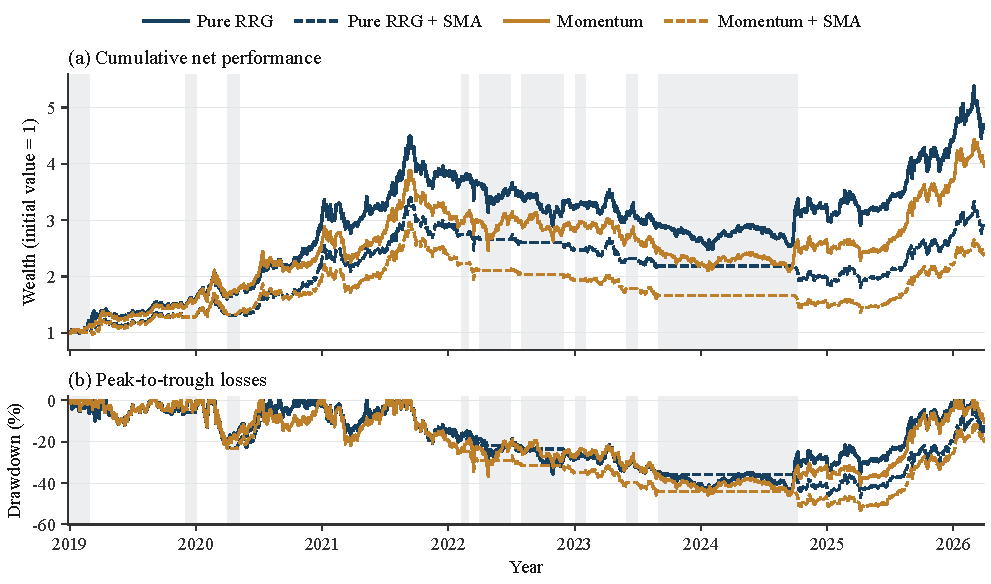
\includegraphics[width=\linewidth,height=.34\textheight,keepaspectratio]{figures/07_sma10.pdf}\caption{Trend-filter comparison. Solid lines denote the original strategies and dashed lines their ten-month moving-average variants. Shading denotes periods in which the common gate allocates the filtered portfolios to cash. Panel (b) reports each portfolio's drawdown relative to its own running maximum.}\end{figure}

In September 2024, the closed gate misses Q's 17.58\% return. Following re-entry on 8 October, filtered Q loses 9.78\% that month, versus a positive 0.53\% for the original. This episode illustrates the sensitivity of a lagged filter to rapid reversals.

\begingroup\footnotesize\setlength{\tabcolsep}{4pt}\renewcommand{\arraystretch}{1.1}

\begin{longtable}{@{}lrrr@{}}

\caption{Dates of maximum drawdown}\\\toprule

Strategy & Peak date & Trough date & Max. DD\\\midrule\endfirsthead

\multicolumn{4}{l}{\textit{Table \thetable\ continued}}\\\toprule

Strategy & Peak date & Trough date & Max. DD\\\midrule\endhead

\midrule\multicolumn{4}{r}{\textit{Continued on next page}}\\\endfoot\bottomrule\endlastfoot

Q & 2021-09-13 & 2024-01-22 & -44.76\%\\

Q+SMA & 2021-09-13 & 2025-04-07 & -47.04\%\\

M & 2021-09-13 & 2024-09-11 & -46.19\%\\

M+SMA & 2021-09-13 & 2025-04-07 & -53.96\%\\

\end{longtable}\endgroup

The electronic supplement provides the complete monthly returns and gate states. Original NAV paths and execution checks reconcile with the archived results.

\clearpage\section{Reproducibility index and supplementary records}\footnotesize\setcounter{table}{0}\setcounter{figure}{0}

The \texttt{tables/} directory accompanying this TeX project contains 19 full-precision CSV files. The tables below identify the complete underlying series as well as the test families. Detailed returns remain available electronically for replication and alternative summaries. The \texttt{figures/} directory contains English vector PDFs and corresponding 300-dpi PNG files. A common typographic and color scheme identifies strategies across all figures.

\begingroup\footnotesize\setlength{\tabcolsep}{4pt}\renewcommand{\arraystretch}{1.1}

\begin{longtable}{@{}lr@{}}

\caption{Complete supplementary CSV inventory}\\\toprule

File & Rows\\\midrule\endfirsthead

\multicolumn{2}{l}{\textit{Table \thetable\ continued}}\\\toprule

File & Rows\\\midrule\endhead

\midrule\multicolumn{2}{r}{\textit{Continued on next page}}\\\endfoot\bottomrule\endlastfoot

\texttt{all\_HAC\_tests.csv} & 18\\

\texttt{annual\_returns.csv} & 9\\

\texttt{benchmark\_adjusted\_regression.csv} & 2\\

\texttt{cost\_pairwise\_tests.csv} & 24\\

\texttt{cost\_sensitivity.csv} & 16\\

\texttt{grid\_multiple\_tests.csv} & 54\\

\texttt{historical\_membership\_coverage.csv} & 10\\

\texttt{main\_performance.csv} & 4\\

\texttt{month\_dependency.csv} & 4\\

\texttt{monthly\_returns\_complete.csv} & 87\\

\texttt{paired\_block\_bootstrap.csv} & 12\\

\texttt{parameter\_grid.csv} & 27\\

\texttt{primary\_pairwise\_tests.csv} & 6\\

\texttt{rolling\_12m\_returns.csv} & 76\\

\texttt{rolling\_summary.csv} & 4\\

\texttt{sma10\_drawdown\_periods.csv} & 4\\

\texttt{sma10\_market\_filter.csv} & 88\\

\texttt{sma10\_monthly\_comparison.csv} & 88\\

\texttt{sma10\_performance.csv} & 4\\

\end{longtable}\endgroup

Main source outputs: \path{results/rrg_tushare_repaired_20261107/}.

Core scripts in the project's \texttt{src/} directory:
\begin{itemize}
\item Data and execution: \path{rrg_repair_inputs.py}; \path{rrg_repair_backtest.py}.
\item Robustness: \path{rrg_report_robustness.py}.
\item Inference and risk control: \path{rrg_report_inference.py}; \path{rrg_sma10_overlay.py}.
\end{itemize}
Audit records cover settings (\path{run.json}), input repair (\path{input_audit.json}), execution (\path{validation.json}), checksums (\path{input_file_hashes.json}) and readback (\path{final_readback.json}).

Input database SHA256:\par
{\scriptsize\texttt{e71a0043112ba173307eac16acbecc1f72c232bb1780ddac455d32c02a407524}}\par
Fixed upstream commit:\par
{\scriptsize\texttt{3f83a77f4c7996ed8185b8979a42c4372c1d811f}}\par
The group's work comprises data integration and repair, extending the first-quadrant rule to ETF allocation, harmonizing implementation and benchmarking, and the additional empirical checks. Signal, exposure, optimization and core execution functions are reused from the pinned implementation.

\subsection*{References and methodological sources}
Western Securities Research Center (2026). \emph{Index-based Allocation Research Series (6): Sector Research under the Relative Rotation Graph Framework}. 25 May. Chinese report.

hugo2046. \emph{QuantsPlaybook}. Fixed version above. \url{https://github.com/hugo2046/QuantsPlaybook}.

Tushare-compatible interface: authorized local data archive. Coverage and definitions are documented in Appendix A.

Faber, M. (2007; updated 2013). \emph{A Quantitative Approach to Tactical Asset Allocation}. The Journal of Wealth Management. Source pointer retained in the existing experiment: \url{https://ssrn.com/abstract=962461}.

\texttt{statsmodels}: HAC-robust covariance and Holm multiple-comparison implementation, as recorded in the local inference scripts. \texttt{arch}: circular time-series block bootstrap implementation, as recorded in the local inference scripts.
\end{document}

